

%---------------------------------------------
%
%       START
%
%---------------------------------------------

\chapter[Spatio-temporal disparity in mammals at the K-Pg boundary]{Spatio-temporal disparity in mammals at the K-Pg boundary}
\label{chap:STD_paper}

\bigskip
\begin{center}

\noindent{\Large \bf Mammalian morphological diversity does not increase in response to the Cretaceous-Paleogene mass extinction and the extinction of the (non-avian) dinosaurs.}
\footnote{A similar version of this chapter has been submitted for publication.}$^{,}$\footnote{\textit{Author contributions}: I designed the study, collected the data, ran the analyses and wrote the paper. NC helped design the study and commented on drafts of the manuscript.} \\

\begin{figure}[h]
  \centering
  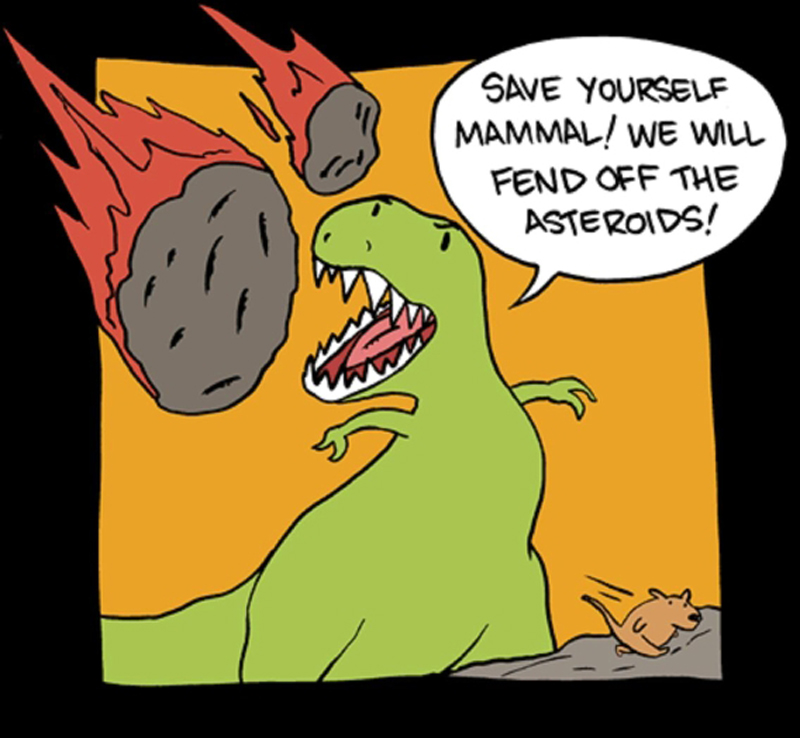
\includegraphics[width=0.8\textwidth]{STD/Figures/SMBC-ZachWeinersmith.jpg}
  \caption*{smbc-comics.com/?id=1535 -- \copyright SMBC Zach Weinersmith}
\end{figure}

\begin{quoteshrink}
  ``The most erroneous stories are those we think we know best - and therefore never scrutinize or question.''
\hfill{S.J. Gould\footnote{Gould, S.J. 1997. \textit{Full House: The Spread of Excellence from Plato to Darwin.} Harmony Books: New York. p 57.}}
\end{quoteshrink}
\bigskip

%} \\
% \medskip
% \noindent Key words: Total Evidence method, data structure, phylogenetic, fossil, topology\\
% \bigskip
% \noindent A shorter version (2500 words) will be submitted to Biology Letters as an invited submission for a special issue on phylogenies with living and fossil species. This special issue is open to submission in December 2015.\\

\end{center}
%---------------------------------------------
%
%       ABSTRACT
%
%---------------------------------------------

\newpage
\section*{Abstract}

Popular science accounts state that after the extinction of the non-avian dinosaurs at the Cretaceous-Paleogene (K-Pg) boundary 66 million years ago, mammals rapidly diversified to fill their empty ecological niches.
However, evidence for this is mixed. 
Palaeontological analyses suggest that mammals radiated in response to the K-Pg extinction event, whereas neontological analyses suggest that mammals began to radiate before K-Pg and were not greatly affected by it. 
Here we aim to end this debate by looking at fossil and living taxa simultaneously.

We investigated the effect of the K-Pg extinction event on mammalian morphological diversity (disparity) using two Total Evidence tip-dated phylogenies of Mammaliaformes and Eutheria, containing both fossil and living taxa. 
Using a novel, continuous time-slicing method for measuring changes in disparity-through-time, we found no significant change in disparity before and after the K-Pg boundary, under either a gradual or punctuated model of evolution.
This implies that the extinctions at the end of the Cretaceous did not affect mammalian morphological evolution. 
Our findings contradict the popular theory that the non-avian dinosaurs and other Mesozoic tetrapods were restricting mammalian evolution, and that their extinction liberated ecological niches for mammals to evolve into.


\newpage 

%---------------------------------------------
%
%       INTRODUCTION
%
%---------------------------------------------

\section{Introduction}
Throughout history, life on Earth has suffered a series of mass extinction events resulting in drastic declines in global biodiversity \citep[e.g.][]{RaupPT,BentonPT,rennetime2013,Brusatte2015}.
The long-term effects of mass extinctions, however, are more varied \citep{Erwin1998344}, and include species richness increases in some clades \citep{friedmanexplosive2010} and declines in others \citep{Benton85}, changes in morphological diversity \citep{Ciampaglio2001,Ciampaglio2004,kornextinction2013} and shifts in ecological dominance \citep[e.g.][]{Brusatte12092008,toljagictriassic-jurassic2013,bensonfaunal2014}.
These shifts are characterised by the decline of one clade that is replaced by a different unrelated clade with a similar ecological role (e.g. Brachiopoda and Bivalvia at the end Permian extinction; \citealt{Liow2015} %Sepkiski1981, CLAPHAM01102006
 but see \citealt{Payne22052014}). 
Shifts in ecological dominance are of particular interest because they are a fairly common pattern observed in the fossil record (e.g. Foraminifera; \citealt{Coxall01042006} %D'Hondt01011996
; Ichtyosauria; \citealt{thorneresetting2011}; Plesiosauria; \citealt{bensonfaunal2014}) and are often linked to major macroevolutionary processes such as adaptive \citep{Losos2010} or competitive \citep{Brusatte12092008} radiations.

One classical example of a shift in ecological dominance is at the Cretaceous-Palaeogene (K-Pg) mass extinction 66 million years ago \citep{rennetime2013}, where many terrestrial vertebrates (including the dominant non-avian dinosaur group; \citealt{archibald2011extinction,rennetime2013,Brusatte2015}) went extinct, allowing placental mammals to dominate the fauna \citep{archibald2011extinction,Lovergrove}. 
Some authors suggest this reflects placental mammals filling the ``empty'' niches left after the K-Pg extinction event \citep{archibald2011extinction,O'Leary08022013}, others suggest it reflects a release from predation and/or competition \citep{Slater2012MEE,Lovergrove}.
However, evidence for the diversification of placental mammals being driven by the K-Pg extinction event is mixed.
Thorough analysis of the fossil record \citep[e.g.][]{goswamia2011,O'Leary08022013} supports the idea that placental mammals diversified after the K-Pg extinction event as there are no undebated placental mammal fossils before it and many afterwards \citep{archibald2011extinction,goswamia2011,Slater2012MEE,O'Leary08022013,Wilson2013,Brusatte2015}. 
Conversely, evidence from molecular data suggests that the diversification of placental mammals started prior to the K-Pg extinction event without being drastically affected by it \citep[e.g.][]{Douady2003285,bininda-emondsthe2007,meredithimpacts2011,Stadler12042011}.
Therefore, whether the diversification of placental mammals began before the K-Pg extinction event, or in response to the extinctions at K-Pg, is a matter of great debate \citep{dosReis2012,O'Leary08022013,Springer09082013,O'Leary08022013,dosReis2014}. 

There are two main reasons why there is still debate about the timing of the diversification of placental mammals. 
Firstly, palaeontological and neontological data show different patterns; palaeontological data generally suggest that placental mammals diversified after K-Pg \citep[e.g.][]{O'Leary08022013}, whereas neontological data suggest that K-Pg extinction event had little to no effect on mammalian diversification \citep{bininda-emondsthe2007,meredithimpacts2011,Stadler12042011}.
We can solve this issue by using both palaeontological and neontological data in our analyses. 
The Total Evidence method allows us to use cladistic data for both living and fossil taxa, along with molecular data for living taxa, to build phylogenies \citep{ronquista2012}. %eernissetaxonomic1993
This method can also be combined with the tip-dating method \citep{ronquista2012,Wood01032013} to get more accurate estimates of diversification times for both fossil and living species \citep[but see][]{Arcila2015131}.
Here we use two recent Total Evidence tip-dated phylogenies of mammals \citep{Slater2012MEE,beckancient2014} to investigate palaeontological and neontological taxa simultaneously.

A second issue is that diversity can be defined in many different ways.
In many studies it is measured as taxonomic diversity or species richness \citep{Stadler12042011,meredithimpacts2011,O'Leary08022013}, but often the more interesting aspect of diversity is related to the ecological niches the species occupy \citep{Wesley-Hunt2005,Brusatte12092008,toljagictriassic-jurassic2013}, particularly if we want to make hypotheses about macroevolutionary processes \citep{Pearman2008149,OlsonRadiation,Losos2010,glor2010phylogenetic,benton2015}.
Sometimes taxonomic diversity is used as a proxy for other kinds of diversity, however, species richness can be decoupled from morphological diversity \citep[e.g.][]{slaterCetacean,ruta2013,hopkinsdecoupling2013}, so it may not be the best proxy for ecological diversity.
We can instead use morphological diversity, also known as disparity \citep[e.g.][]{Wills1994,Erwin2007,Hughes20082013}, as a way to quantify changes in mammalian morphology that should relate to the ecology of the species.
However some methods for measuring disparity are outdated and make inappropriate assumptions.
Many methods for quantifying changes in morphological diversity were proposed $>$ 20 years ago \citep{Foote01071994,Wills1994} and are sometimes used without modifications \citep[e.g.,][]{brusatte50,Brusatte12092008,cisneros2010,thorneresetting2011,prentice2011,brusattedinosaur2012,toljagictriassic-jurassic2013,ruta2013,bentonmodels2014,bensonfaunal2014}.
Additionally, previous methods are based on an underlying assumption that changes in disparity occur by punctuated evolution \citep[e.g.][]{Wesley-Hunt2005} which is not always the case \citep{Hunt21042015}.
Finally, most studies of disparity through time use unequal time units based on biostratigraphy \citep{Brusatte12092008,brusattedinosaur2012,toljagictriassic-jurassic2013}. 
This can be tautological as biostratigraphy is already based on changes in fossil assemblages and morphology through time.
To deal with these issues, we propose an updated approach to test whether mammals diversified in response to the K-Pg event, using morphological disparity, measured as cladistic disparity (see Methods), as our proxy for diversity.

Here we measure the disparity of living and fossil mammals before or after K-Pg, using data taken from two previously published studies \citep{Slater2012MEE,beckancient2014}. 
Using a novel time-slicing approach, we produce fine-grained estimates of disparity through time under two different models of morphological character evolution (either gradual or punctuated). 
We also test whether mammals display significant changes in disparity between the end of the Cretaceous and throughout the Cenozoic.

Until now, this question has only been investigated using data from North American Therian mammals (excluding Monotremata) and without formally testing the effect of the K-Pg extinction event \citep{Wilson2013}.
To our knowledge, this study is the first to approach the debate about the effects of the K-Pg extinction event on mammalian evolution using Total Evidence phylogenies and by calculating disparity through time in a continuous way.
We find no significant changes in mammalian disparity between the end of the Cretaceous and any time during the Paleocene. 
These results suggest that the extinction of non-avian dinosaurs and other terrestrial vertebrate clades at the end of the Cretaceous did not affect mammalian morphological evolution.

%---------------------------------------------
%
%       METHODS
%
%---------------------------------------------

\section{Methods}

\subsection{Cladistic data and phylogenies}
We used the cladistic morphological matrices and the Total Evidence tip-dated trees \citep{ronquista2012} from \citet[][103 taxa with 446 morphological characters;]{Slater2012MEE} and \citet[][102 taxa with 421 morphological characters]{beckancient2014}.
We chose these two datasets because they have a similar number of taxa and morphological characters.
\cite{Slater2012MEE} ranges from 310 million years ago (Ma; Late Carboniferous) to the present and focuses on the clade Mammaliaformes at the family-level and is called hereafter the Mammaliaformes dataset.
\cite{beckancient2014} ranges from 170 Ma (Middle Jurassic) to the present and focuses on Eutheria at the genus-level and is called hereafter the Eutheria dataset.
We used the first and last occurrences reported in \cite{Slater2012MEE} and \cite{beckancient2014} as the temporal range of each taxon in our analysis.
Both phylogenies are illustrated in the supplementary material (see Fig \ref{fig:SlaterTree} and \ref{fig:BeckTree}).
Both trees contain few taxa compared to the overall species richness of living and fossil mammals \citep{bininda-emondsthe2007,archibald2011extinction}.
This is because Total Evidence trees need a lot of data, particularly morphological data for living taxa that can be hard to locate \citep{GuillermeCooper}.
Therefore, most Total Evidence studies to date contain one or two orders of magnitude fewer taxa than phylogenies based solely on molecular data (e.g. thousands of taxa in \citealt{bininda-emondsthe2007,meredithimpacts2011} \textit{vs.} hundreds in \citealt{ronquista2012,Slater2012MEE,Wood01032013,beckancient2014}).

\begin{figure}[!h]
\centering
    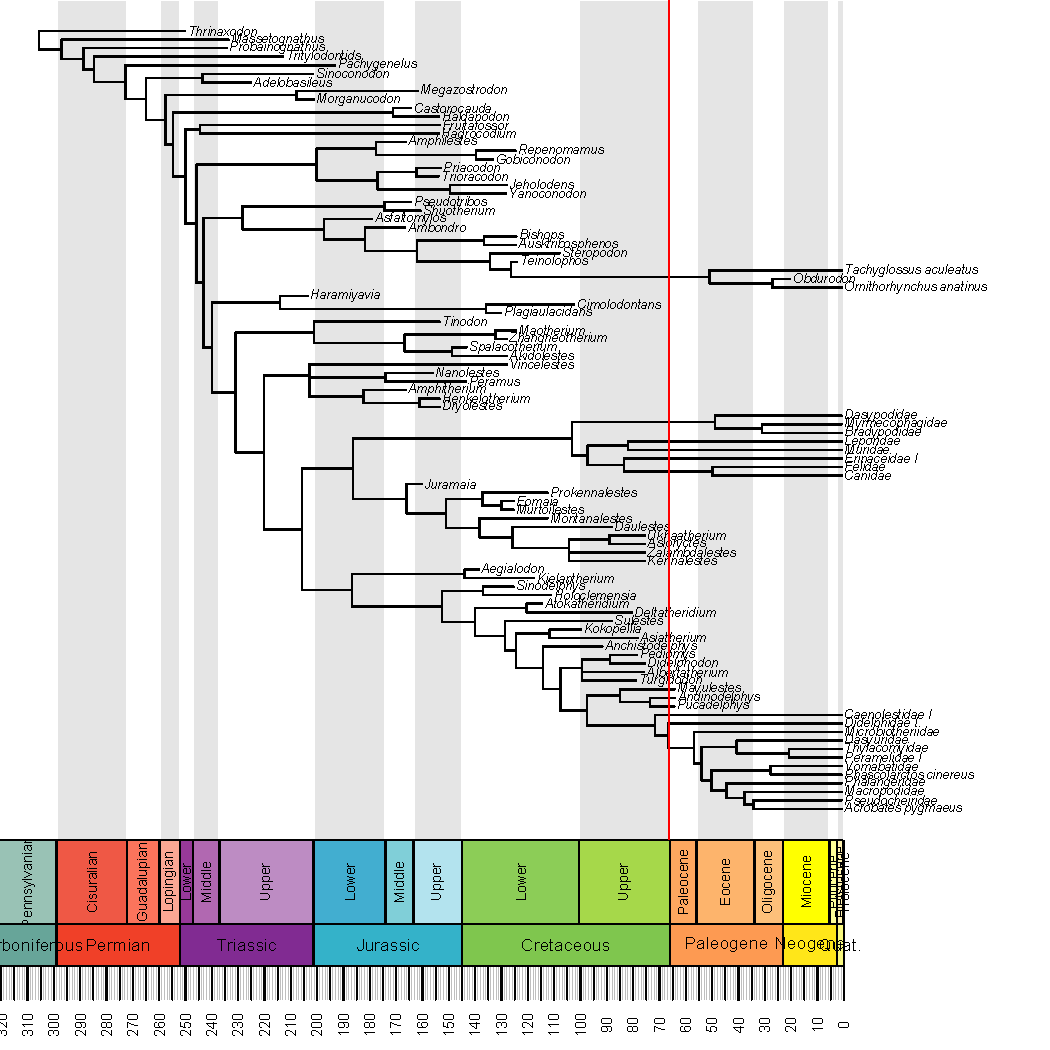
\includegraphics[keepaspectratio=true]{STD/Figures/Slater_tree.pdf}
\caption[Mammaliaformes phylogeny]{Mammaliaformes phylogeny from \cite{Slater2012MEE}. The phylogeny only contains taxa with overlapping cladistic data. The vertical red line represents the K-Pg boundary. Carb. = Carboniferous; Quat. = Quaternary.}
\label{fig:SlaterTree}
\end{figure}

\begin{figure}[!h]
\centering
    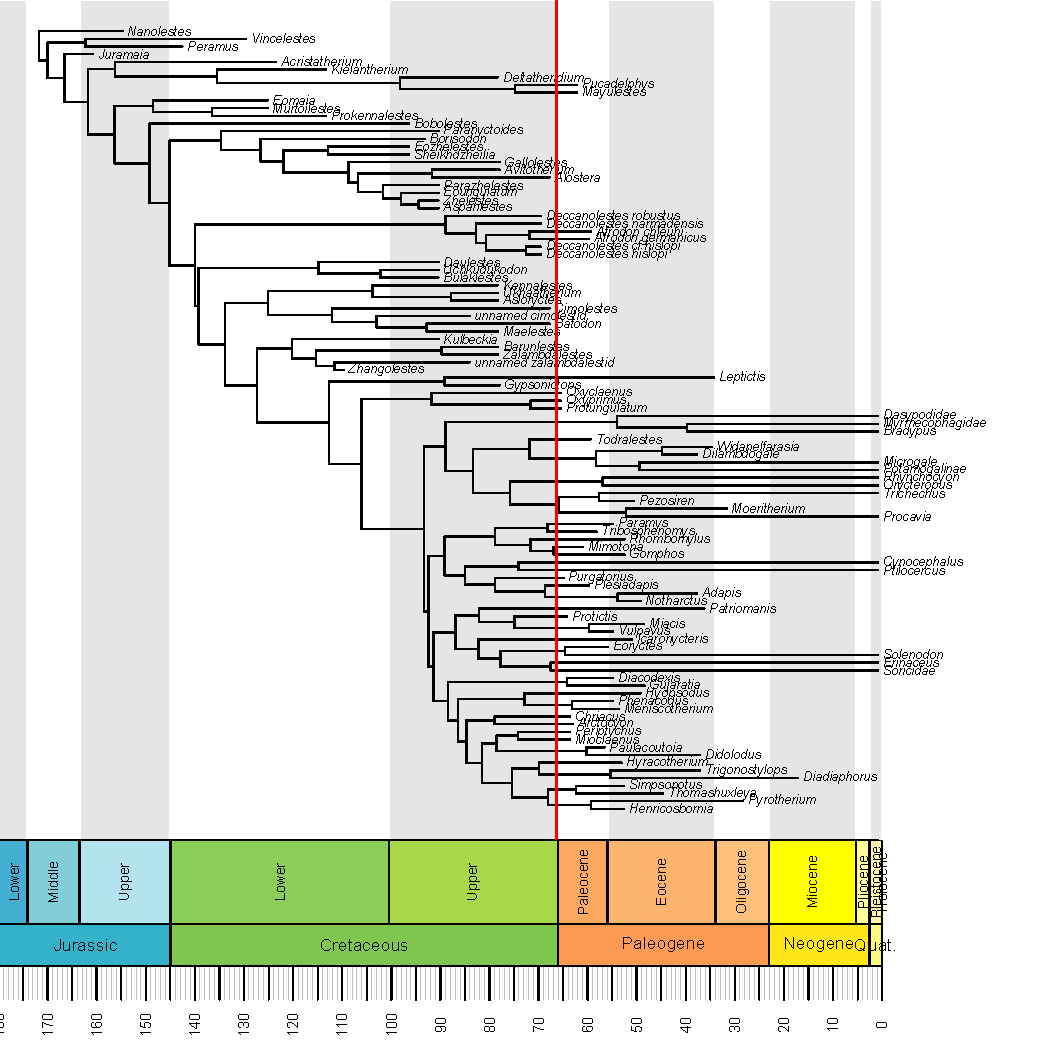
\includegraphics[keepaspectratio=true]{STD/Figures/Beck_tree.pdf}
\caption[Eutheria phylogeny]{Eutheria phylogeny from \cite{beckancient2014}. The phylogeny only contains taxa with overlapping cladistic data. The vertical red line represents the K-Pg boundary. Quat. = Quaternary.}
\label{fig:BeckTree}
\end{figure}

\subsection{Estimating ancestral character states}
For both datasets we used the re-rooting method \citep{Yang01121995,Garland2000} to get Maximum Likelihood estimates of the ancestral states for each character at every node in the tree, using the \texttt{rerootingMethod} function from the \texttt{R} package \texttt{phytools} version 0.4-45 \citep{phytools,R}.
Where there was missing character data for a taxon we followed the method of \cite{Claddis} and treated missing data as any possible observed state for each character.
For example, if a character had two observed states ($0$ and $1$) across all taxa, we attributed the multi-state ``$0$\&$1$" value to the taxon with missing data, representing an equal probability of being either $0$ or $1$.
This allows the ancestral node of a taxon with missing data to be estimated with no assumptions other than that the taxon has one of the observed character states.
To prevent poor ancestral state reconstructions from biasing our results, especially when a lot of error is associated with the reconstruction, we only included ancestral state reconstructions with a scaled Likelihood $\geq$ $0.95$.
Ancestral state reconstructions with scaled Likelihoods below this threshold were replaced by missing data (``?'').

\subsection{Building the cladisto-space}
To explore variations in mammalian disparity through time (defined here as the variation in morphologies through time), we used a cladisto-space approach \citep[e.g.][]{Foote01071994,Foote29111996,Wesley-Hunt2005,Brusatte12092008,friedmanexplosive2010,toljagictriassic-jurassic2013,Hughes20082013}.
This approach is similar to constructing a morphospace based on continuous morphological data \citep[e.g.][]{friedmanexplosive2010}, except a cladisto-space is an approximation of the morphospace based on cladistic data (i.e. the discrete morphological characters used to build a phylogenetic tree).
Mathematically, a cladisto-space is an $n$ dimensional object that summarises the cladistic distances between the taxa present in a cladistic matrix (see details below).
Although empirically inter-taxon distances are the same in a morphospace or a cladisto-space \citep{foth2012different,hetherington2015cladistic}, we prefer the term cladisto-space to make it clear that this space is estimated using cladistic data and not morphometric data and because both objects have slightly different properties.
For example, because of its inherent combinatory properties, a cladisto-space is a finite theoretical object limited by the product of the number of character states, whereas a morphospace is an infinite theoretical object.
Thus a cladisto-space will be overloaded if the number of taxa is higher than the product of the number of character states, although this is rarely an issue with empirical data (our cladisto-spaces have maximal capacities of $1.9$$\times$$10^{181}$ taxa for the Mammaliaformes dataset, i.e. 101 orders of magnitude more taxa than the number of particles in the universe; and $4.5$$\times$$10^{159}$ taxa for the Eutheria dataset).

To estimate the cladisto-spaces for each of our datasets we first constructed pairwise distance matrices of length $k$, where $k$ is the total number of tips and nodes in the datasets.
For each dataset separately, we calculated the $k$$\times$$k$ distances using the Gower distance \citep{Gower71}, i.e. the Euclidean distance between two taxa divided by the number of shared characters. 
This allows us to correct for distances between two taxa that share many characters and could be closer to each other than to taxa with fewer characters in common (i.e. because some pairs of taxa share more characters in common than others, they are more likely to be similar).
For cladistic matrices, using this corrected distance is preferable to the raw Euclidean distance because of its ability to deal with discrete or/and ordinated characters as well as with missing data \citep{anderson2012using}.
However, the Gower distance cannot calculate distances when taxa have no overlapping data.
Therefore, we used the \texttt{TrimMorphDistMatrix} function from the \texttt{Claddis} R package \citep{Claddis} to remove pairs of taxa with no cladistic characters in common.
This led to us removing 11 taxa from the Mammaliaformes dataset but none from the Eutheria dataset.

%\subsubsection{Ordination}
After calculating our distance matrices we transformed them using classical multidimensional scaling \citep[MDS;][]{torgerson1965multidimensional,GOWER01121966,cailliez1983analytical}.
This method (also referred to as PCO; e.g. \citealt{Brusatte2015}; or PCoA; e.g. \citealt{paradisape:2004}) is an eigen decomposition of the distance matrix.
Because we used Gower distances instead of raw Euclidean distances, negative eigenvalues can be calculated.
To avoid this problem, we first transformed the distance matrices by applying the Cailliez correction \citep{cailliez1983analytical} which adds a constant $c^*$ to the values in a distance matrix (apart from the diagonal) so that all the Gower distances become Euclidean ($d_{Gower}+c^*=d_{Euclidean}$; \citealt{cailliez1983analytical}). 
We were then able to extract $n$ eigenvectors for each matrix (representing the $n$ dimensions of the cladisto-space) where $n$ is equal to $k-2$, i.e. the number of taxa in the matrix ($k$) minus the last two eigenvectors that are always null after applying the Cailliez correction.
Contrary to previous studies \citep[e.g][]{brusatte50,cisneros2010,prentice2011,anderson2012using,Hughes20082013,bentonmodels2014}, we use all $n$ dimensions of our cladisto-spaces and not a subsample representing the majority of the variance in the distance matrix (e.g. selecting only $m$ dimensions that represent up to 90\% of the variance in the distance matrix; \citealt{Brusatte12092008,toljagictriassic-jurassic2013}).

Note that our cladisto-spaces represent an ordination of all possible mammalian morphologies coded in each study through time.
It is unlikely that all morphologies will co-occur at each time point, therefore, the disparity of the whole cladisto-space is expected to be greater than the disparity at any specific point in time.

\subsection{Calculating disparity}
Disparity can be estimated in many different ways \citep[e.g.][]{Wills1994,Ciampaglio2004,thorneresetting2011,hopkinsdecoupling2013,huang2015origins}, however most studies estimate disparity using four metrics: the sum and products of ranges and variances, each of which gives a slightly different estimate of how the data fits within the cladisto-space \citep{Foote01071994,Wills1994,brusatte50,Brusatte12092008,cisneros2010,thorneresetting2011,prentice2011,brusattedinosaur2012,toljagictriassic-jurassic2013,ruta2013,bentonmodels2014,bensonfaunal2014}.
Nonetheless, these methods suffer several methodological caveats.
First, the range metrics are affected by the uneven sampling of the fossil record \citep{Butler2012}
Second, because we include all $n$ dimensions in the analysis (see above), the products of ranges and variances will tend towards zero since the scores of the last dimension are usually really close to zero themselves. 
These features make using the sum and products of ranges and variances unfeasible in our study.
Instead, we use a different metric that comes with no statistical assumptions for measuring the dispersion of the data in the cladisto-space: the median distance between tips and nodes and the centroid (similar but not equivalent to \citealt{Wills1994,kornextinction2013,huang2015origins}) calculated as:

\begin{equation}
   Disparity=median{\displaystyle\sqrt{\sum{(\mathbf{v}_{n}-Centroid_{n})^2}}}
    \label{disparity}
\end{equation}
where:
\begin{equation}
    Centroid_{n}=\frac{\displaystyle\sum(\mathbf{v}_{n})}{k} 
    \label{centroid}
\end{equation}

\noindent
and $\mathbf{v}_{n}$ is any of the $n$ eigenvectors (i.e. any of the $n$ dimensions of the cladisto-space), $Centroid_{n}$ is the mean value of the $n^{th}$ eigenvector (equation \ref{centroid}) and $k$ is the total number of tips and nodes.
Note that we also calculated the sum and products of ranges and variances and refer to these results in the appendix \ref{chap:Appendix_STD} (Fig \ref{Supp_disparity_all_Mammaliaformes}, \ref{Supp_disparity_all_Eutheria}, \ref{Supp_disparity_all_Mammaliaformes_rarefied}, \ref{Supp_disparity_all_Eutheria_rarefied}). % link to supp.

\subsection{Estimating disparity through time} 
Changes in disparity through time are generally investigated by calculating the disparity of taxa that occupy the cladisto-space during specific time intervals \citep[e.g][]{cisneros2010,prentice2011,Hughes20082013,hopkinsdecoupling2013,bentonmodels2014,bensonfaunal2014}.
These time intervals are usually defined based on biostratigraphy \citep[e.g.][]{cisneros2010,prentice2011,Hughes20082013,bentonmodels2014} but can also be arbitrarily chosen time periods of equal duration \citep{Butler2012,hopkinsdecoupling2013,bensonfaunal2014}.
However, this approach suffers from two main biases. 
First, if biostratigraphy is used to determine the time intervals, disparity may be distorted towards higher differences between time intervals because biostratigraphical periods are geologically defined based on differences in the morphology of fossils found in the different strata.
Second, this approach assumes that all characters evolve following a punctuated equilibrium model, because disparity is only estimated once for each interval resulting in all changes in disparity occurring between intervals, rather than also allowing for gradual changes within intervals \citep{Hunt21042015}.

To address these issues, we used a ``time-slicing'' approach that considers subsets of taxa in the cladisto-space at specific equidistant points in time, as opposed to considering subsets of taxa between two points in time.
This results in even-sampling of the cladisto-space across time and permits us to define the underlying model of character evolution (punctuated or gradual).  
In practice, time-slicing considers the disparity of any element present in the phylogeny (branches, nodes and tips) at any point in time.
When the phylogenetic elements are nodes or tips, the eigenvector scores for the nodes (estimated using ancestral state reconstruction as described above) or tips are directly used for estimating disparity.
When the phylogenetic elements are branches we chose the eigenvector score for the branch using one of two evolutionary models:
\begin{enumerate}
    \item{\textbf{Punctuated evolution.}} 
    This model selects the eigenvector score from either the ancestral node or the descendant node/tip of the branch regardless of the position of the slice along the branch. 
    Similarly to the time interval approach, this reflects a model of punctuated evolution where changes in disparity occur either at the start or at the end of a branch over a relatively short time period and clades undergo long periods of stasis during their evolution \citep{Gould1977,Hunt20112007}.
    We applied this model in three ways: 
    \begin{enumerate}[(i)]
      \item selecting the eigenvector score of the ancestral node of the branch (ACCTRAN).
      \item selecting the eigenvector score of the descendant node/tip of the branch (DELTRAN).
      \item randomly selecting either the eigenvector score of the ancestral node or the descendant node/tip of the branch (random).
    \end{enumerate}
    Method (i) assumes that changes always occur early on the branch (accelerated transition, ACCTRAN) and (ii) assumes that changes always occur later (delayed transition, DELTRAN).
    We prefer not to make either assumption so we report the results from (iii), although the ACCTRAN and DELTRAN results are available in the appendix \ref{chap:Appendix_STD} (Fig \ref{Supp_disparity_all_Mammaliaformes}, \ref{Supp_disparity_all_Eutheria}, \ref{Supp_disparity_all_Mammaliaformes_rarefied}, \ref{Supp_disparity_all_Eutheria_rarefied}).
    \item{\textbf{Gradual evolution.}}
    This model also selects the eigenvector score from either the ancestral node or the descendant node/tip of the branch, but the choice depends on the distance between the sampling time point and the end of the branch.
    If the sampling time point falls in the first half of the branch length the eigenvector score is taken from the ancestral node, conversely, if the sampling time point falls in the second half of the branch length the eigenvector score is taken from the descendant node/tip.
    This reflects a model of gradual evolution where changes in disparity are gradual and cumulative along the branch.
    Under this model, the gradual changes could be either directional or random, however, directional evolution have been empirically shown to be rare \citep[only 5\% of the time][]{Hunt20112007}.
    We therefore considered that changes from a character state A to B were only dependent on the branch length.
\end{enumerate}
%What did we do (the main figure)
We applied our time-slicing approach separately to the two cladisto-spaces calculated for the Mammaliaformes and Eutheria datasets, time-slicing the phylogeny every five million years from 170 Ma to the present resulting in 35 subsamples of the cladisto-space.
For each subsample, we estimated its disparity assuming punctuated (ACCTRAN, DELTRAN and random) and gradual evolution as described above.
To reduce the influence of outliers on our disparity estimates, we bootstrapped each disparity measurement by randomly resampling with replacement a new subsample of taxa from the observed taxa in the subsample 1000 times.
We then calculated the median disparity value for each subsample along with the 50\% and 95\% confidence intervals.
We also recorded the number of phylogenetic elements (nodes and tips) in each subsample as a proxy for taxonomic diversity.
To compare our results to previous studies we also repeated our analyses using the time interval approach based on biostratigraphy \citep[e.g.][]{cisneros2010,prentice2011,Hughes20082013,bentonmodels2014} using each geological stage from the Middle Jurassic to the present.
We report the results of these analyses in the appendix \ref{chap:Appendix_STD} (Fig \ref{Supp_disparity_all_Mammaliaformes}, \ref{Supp_disparity_all_Eutheria}, \ref{Supp_disparity_all_Mammaliaformes_rarefied}, \ref{Supp_disparity_all_Eutheria_rarefied}).

%Testing the difference section
\subsection{Testing the effects of the K-Pg extinction event on mammalian disparity}
If the K-Pg extinction event had a significant effect on mammalian disparity, we should see a significant difference between disparity at the end of the Cretaceous and disparity at the start of the Paleogene.
To test this, we performed \textit{t}-tests to look for differences in disparity between the time subsamples of interest \citep[e.g. as used in][]{anderson2012using,zelditch2012geometric,smith2014joined}.
We compared the last time subsample before the K-Pg boundary (70 Ma) to the first subsample of the Paleocene (65 Ma) for both the Mammaliaformes and Eutheria datasets and using both the gradual and punctuated evolutionary models.
Even though one million year after the K-Pg event (66 to 65 Ma) seems to be a rather short geological time frame, effects on mammalian evolution have been detected as early as half a million year after K-Pg \citep{Wilson2013}.
However, the effect of extinction on a group's evolution might not be detectable directly after the event due to delays in recovery \citep[e.g.][estimated that ecosystems only fully recovered 8-9 Ma after the Permo-Triassic mass extinction]{chen2012timing}.
Therefore, we also tested whether there was a significant difference in disparity between the end of the Cretaceous (70 Ma) and all subsamples from the Paleocene (65, 60 and 55 Ma).
Additionally, some authors argue that the major diversification event in mammals took place during the Paleocene-Eocene Thermal Maximum (PETM; $\sim$ 56 Ma; \citealt{bininda-emondsthe2007} but see \citealt{meredithimpacts2011} and \citealt{Stadler12042011}) with the extinctions at K-Pg providing the ``empty'' ecological space required for this diversification to occur.
We therefore extended our comparisons between the last subsample of the Cretaceous (70 Ma) up to the late Eocene (35 Ma) to check for a delayed effect of the K-Pg extinction potentially allowing morphological diversification after the PETM. 
Because these analyses involved multiple comparisons, we used Bonferonni corrections \citep{holm1979simple} to ensure our significant results were robust to Type I error rate inflation. 

Finally, disparity may be higher in subsamples with more phylogenetic elements simply because there are more taxa represented.
To test whether this influenced our results, we repeated the \textit{t}-tests using the rarefied Mammaliaformes and Eutheria disparities.
In the Mammaliaformes, the minimum number of taxa in each subsample from 170 Ma to present was eight.
In the Eutheria, the minimum number of taxa in each subsample was three, however, from 150 Ma until the present, the minimum number of taxa is eight.
To make both datasets comparable, we used eight as a minimum number of taxa for the rarefied bootstrap measurements, therefore in the Eutheria we ignored the subsample between 170 and 150 Ma that only contains three taxa.

%---------------------------------------------
%
%       RESULTS
%
%---------------------------------------------

\section{Results}
Disparity in the Mammaliaformes reaches a plateau during the Middle Triassic around 240 Ma, and fluctuates slightly around this during the rest of the Mesozoic and the Cenozoic (Fig \ref{fig:Fig_Raw_results} and Fig \ref{Supp_Mammaliaformes_rarefied}).
The number of tips and nodes in each time subsample (a proxy for taxonomic richness), however, show a more idiosyncratic pattern with a steady increase until the Middle Jurassic around 170 Ma (Fig S5) followed by random fluctuations during the rest of the Mesozoic and the Cenozoic (Fig \ref{fig:Fig_Raw_results}).
Disparity in the Eutheria reaches a plateau at the end of the Jurassic around 150 Ma, whereas the number of tips and nodes increases up to the K-Pg boundary and then decreases throughout the Cenozoic (Fig \ref{fig:Fig_Raw_results}).
For both Mammaliaformes and Eutheria the same patterns in changes in disparity appear in the rarefied analyses (Fig \ref{fig:Fig_Raw_results} and \ref{fig:Fig_Rar_results}).
In both datasets the two evolutionary models (gradual or punctuated) also yield similar results (Fig \ref{fig:Fig_Raw_results}).

We found no significant differences in disparity between the last subsample of the Cretaceous (70 Ma) and the first subsample of the Paleogene (65 Ma; Table \ref{tab:Tab_results}), using both datasets and under both evolutionary models. 
We also found no significant differences in disparity between the last subsample of the Cretaceous (70 Ma) and any subsamples of the Paleocene and Eocene in Mammaliaformes under both evolutionary models and in Eutheria under a gradual evolutionary model (Table \ref{tab:Tab_results}).
However, in Eutheria under the punctuated evolutionary model, we found a small significant difference (after applying Bonferonni corrections) in disparity between the last subsample of the Cretaceous (70 Ma) and the subsamples at 45 Ma (an increase in disparity of 0.17; Table \ref{tab:Tab_results}).
However, this result is not significant in the rarefied analyses (Table \ref{tab:Tab_rare}). 
Otherwise the results of the rarefied analyses are the same as when using the complete datasets. 

\begin{figure}[!htbp]
\centering
    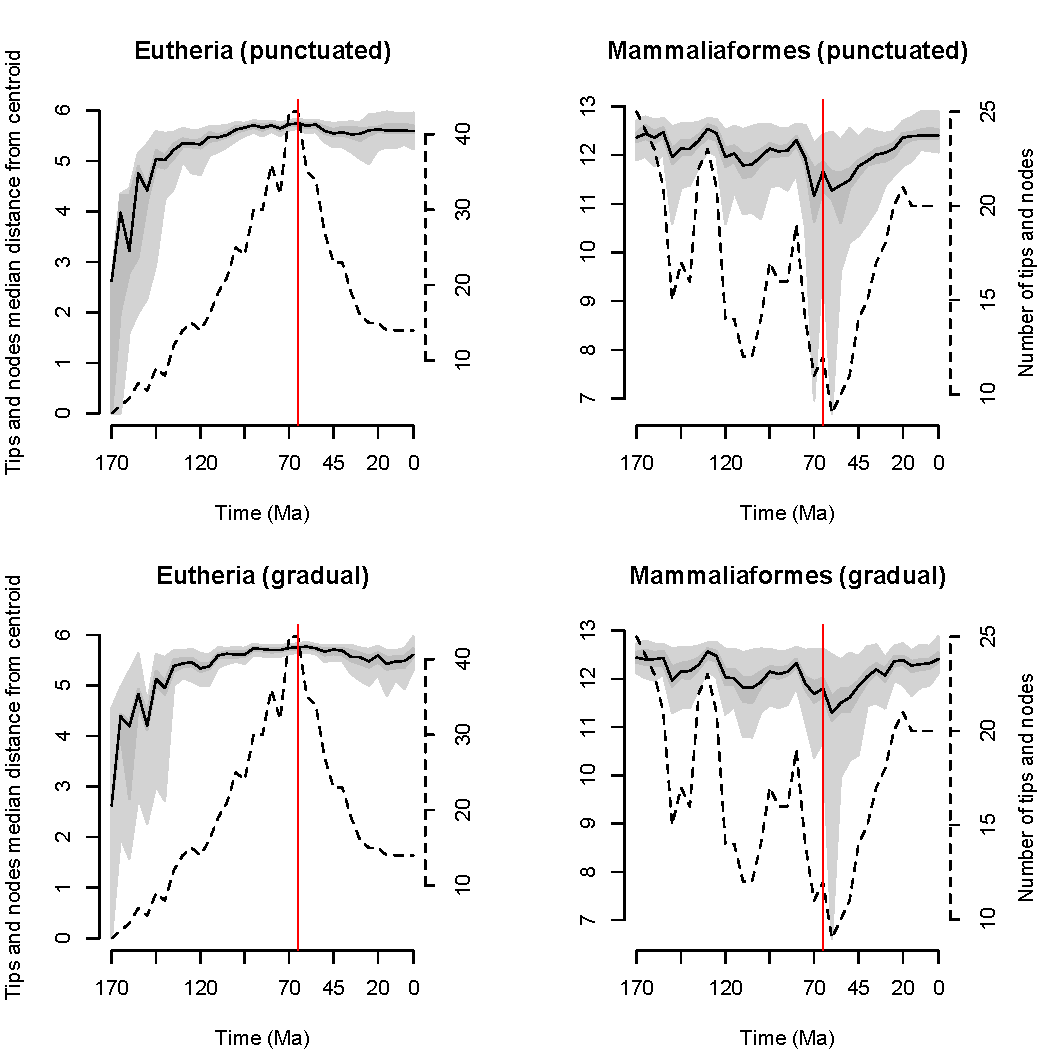
\includegraphics[keepaspectratio=true]{STD/Figures/Main_results.pdf}
\caption[Disparity through time in Eutheria and Mammaliaformes]{Disparity through time in Eutheria and Mammaliaformes calculated using a model of punctuated (upper panels) or gradual (lower panels) evolution. The x axis represents time in millions of years before the present (Ma). The y axis represents disparity, measured as the median distance between the centroid of the ordinated space and the tips/nodes in each time subsample. The solid black lines show the mean disparity estimated from 1000 bootstrapped pseudoreplicates and confidence intervals (CI) are represented by the grey polygons (50\% CI in dark grey and 95\% CI in light grey). The dashed line and the right hand axis represents the number of tips/nodes in each time slice. The red vertical line indicates the Cretaceous-Paleogene (K-Pg) boundary (66 Ma). Note that scale bars differ among panels.}
\label{fig:Fig_Raw_results}
\end{figure}

\begin{figure}[!h]
\centering
    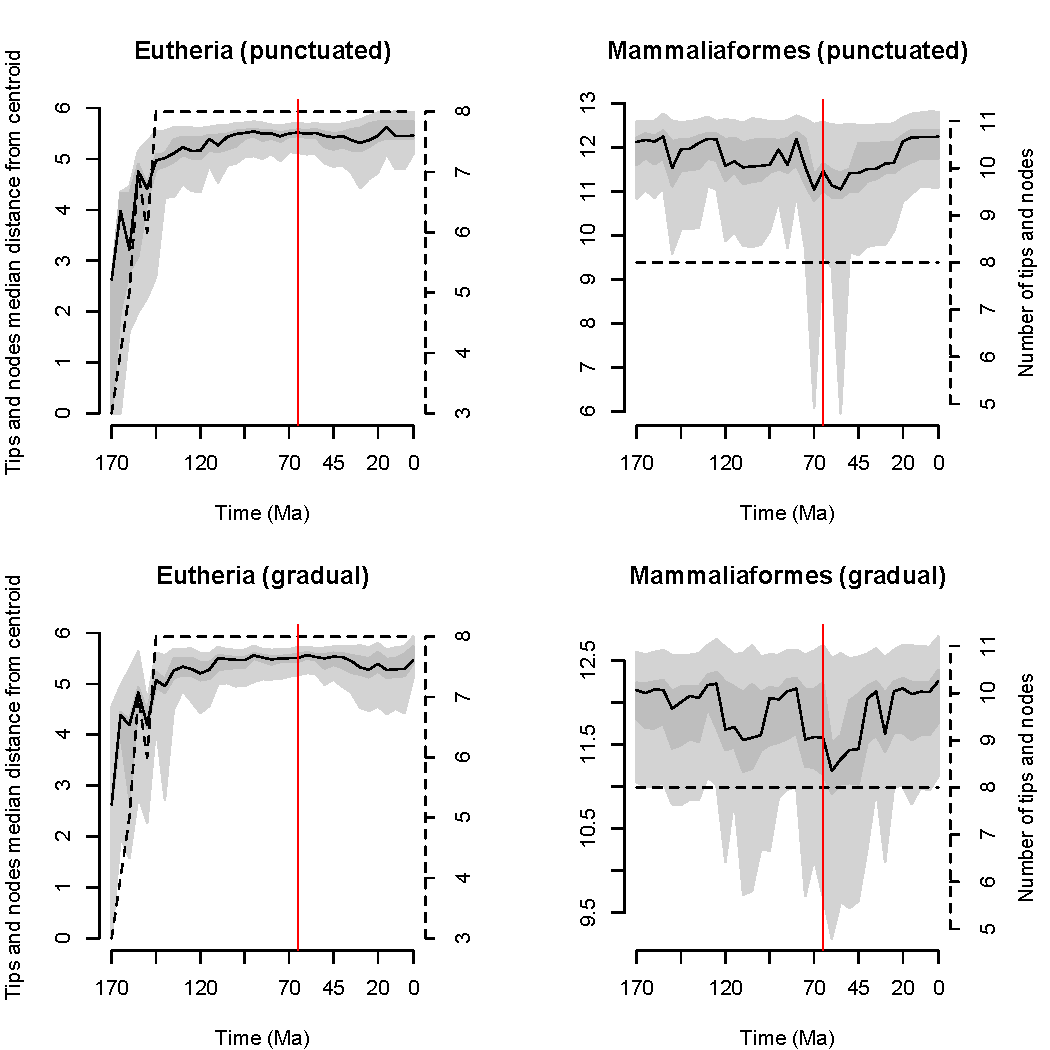
\includegraphics[keepaspectratio=true]{STD/Figures/Main_results_rarefied.pdf}
\caption[Disparity through time in Eutheria and Mammaliaformes (rarefied)]{Rarefied disparity through time in Eutheria and Mammaliaformes calculated using a model of punctuated (upper panels) or gradual (lower panels) evolution. The x axis represents time in millions of years before the present (Ma). The y axis represents disparity, measured as the median distance between the centroid of the ordinated space and the tips/nodes in each time subsample. The solid black lines show the mean disparity estimated from 1000 bootstrapped pseudoreplicates and confidence intervals (CI) are represented by the grey polygons (50\% CI in dark grey and 95\% CI in light grey). The dashed line and the right hand axis represents the number of tips/nodes in each time slice. The red vertical line indicates the Cretaceous-Paleogene (K-Pg) boundary (66 Ma). Note that scale bars differ among panels.}
\label{fig:Fig_Rar_results}
\end{figure}


\begin{table}[ht]
\caption[Effect of the K-Pg boundary on mammlian disparity]{Results of \textit{t}-tests comparing disparity at the last subsample of the Cretaceous (70 Ma) to subsamples of the Paleocene and Eocene, under both gradual and punctuated evolutionary models, in Mammaliaformes and Eutheria. Difference = mean difference in disparity between the two subsamples being compared; df = degrees of freedom; p value = original p value prior to Bonferonni correction. Significant differences (after applying Bonferonni corrections for multiple comparisons) are highlighted in bold.}
\label{tab:Tab_results}
\centering
\begin{tabular}{c|cccc|cccc}
  \hline
  \textbf{Subsamples} & \multicolumn{4}{c|}{\textbf{Gradual evolution model}} & \multicolumn{4}{c}{\textbf{Punctuated evolution model}} \\
  \textbf{compared} & \textbf{difference} & \textbf{df} & \textbf{t} & \textbf{p value} & \textbf{difference} & \textbf{df} & \textbf{t} & \textbf{p value} \\ 
  \hline
  \multicolumn{9}{c}{\textbf{Mammaliaformes}}\\
  \hline
  70 \textit{vs.} 65 & -0.420 & 21 & -0.808 & 0.428 & -0.030 & 21 & -0.058 & 0.954 \\ 
  70 \textit{vs.} 60 & 0.030 & 18 & 0.046 & 0.964 & 0.210 & 18 & 0.379 & 0.709 \\ 
  70 \textit{vs.} 55 & 0.010 & 19 & 0.021 & 0.983 & 0.110 & 19 & 0.225 & 0.824 \\ 
  70 \textit{vs.} 50 & -0.260 & 20 & -0.456 & 0.653 & 0.030 & 20 & 0.060 & 0.953 \\ 
  70 \textit{vs.} 45 & -0.430 & 23 & -0.869 & 0.394 & 0.060 & 23 & 0.132 & 0.896 \\ 
  70 \textit{vs.} 40 & -0.620 & 24 & -1.388 & 0.178 & -0.410 & 24 & -1.031 & 0.313 \\ 
  70 \textit{vs.} 35 & -0.730 & 26 & -1.742 & 0.093 & -0.340 & 26 & -0.861 & 0.397 \\ 
  \hline
  \multicolumn{9}{c}{\textbf{Eutheria}}\\
  \hline
  70 \textit{vs.} 65 & -0.020 & 84 & -0.503 & 0.616 & 0.010 & 84 & 0.288 & 0.774 \\ 
  70 \textit{vs.} 60 & 0.030 & 76 & 0.617 & 0.539 & 0.080 & 76 & 1.693 & 0.095 \\ 
  70 \textit{vs.} 55 & 0.030 & 75 & 0.519 & 0.605 & 0.030 & 75 & 0.699 & 0.486 \\ 
  70 \textit{vs.} 50 & 0.130 & 68 & 2.101 & 0.039$^1$ & 0.080 & 68 & 1.458 & 0.149 \\ 
  70 \textit{vs.} 45 & 0.190 & 64 & 2.679 & 0.009$^1$ & 0.170 & 64 & 2.730 & \textbf{0.006}$^2$ \\ 
  70 \textit{vs.} 40 & 0.160 & 64 & 2.249 & 0.028$^1$ & 0.130 & 64 & 2.084 & 0.041$^1$ \\ 
  70 \textit{vs.} 35 & 0.190 & 60 & 2.358 & 0.022$^1$ & 0.120 & 60 & 1.893 & 0.063 \\ 
   \hline
\end{tabular} \\
   \small{$^1$p value is non-significant after applying Bonferonni correction;
   $^2$p value is \textbf{0.048} after applying Bonferonni correction.}
\end{table}

\begin{table}[ht]
\caption[Effect of the K-Pg boundary on mammlian disparity (rarefied)]{Results of rarefied t-tests comparing disparity at the last subsample of the Cretaceous (70 Ma) to subsamples of the Paleocene and Eocene, under both gradual and punctuated evolutionary models, in Mammaliaformes and Eutheria. Difference = mean difference in disparity between the two subsamples being compared; df = degrees of freedom; p value = original p value prior to Bonferonni correction.}
\label{tab:Tab_rare}
\centering
\begin{tabular}{c|cccc|cccc}
  \hline
  \textbf{Subsamples} & \multicolumn{4}{c|}{\textbf{Gradual evolution model}} & \multicolumn{4}{c}{\textbf{Punctuated evolution model}} \\
  \textbf{compared} & \textbf{difference} & \textbf{df} & \textbf{t} & \textbf{p value} & \textbf{difference} & \textbf{df} & \textbf{t} & \textbf{p value} \\ 
  \hline
  \multicolumn{9}{c}{\textbf{Mammaliaformes}}\\
  \hline
  70 \textit{vs.} 65 & -0.360 & 21 & -0.486 & 0.632 & 0.040 & 21 & 0.054 & 0.957 \\ 
  70 \textit{vs.} 60 & -0.080 & 18 & -0.099 & 0.922 & 0.060 & 18 & 0.094 & 0.927 \\ 
  70 \textit{vs.} 55 & -0.090 & 19 & -0.110 & 0.914 & 0.050 & 19 & 0.082 & 0.936 \\ 
  70 \textit{vs.} 50 & -0.270 & 20 & -0.368 & 0.717 & 0.030 & 20 & 0.041 & 0.968 \\ 
  70 \textit{vs.} 45 & -0.310 & 23 & -0.419 & 0.679 & 0.200 & 23 & 0.285 & 0.778 \\ 
  70 \textit{vs.} 40 & -0.460 & 24 & -0.680 & 0.503 & -0.240 & 24 & -0.422 & 0.677 \\ 
  70 \textit{vs.} 35 & -0.510 & 26 & -0.742 & 0.465 & -0.100 & 26 & -0.159 & 0.875 \\ 
  \hline
  \multicolumn{9}{c}{\textbf{Eutheria}}\\
  \hline
  70 \textit{vs.} 65 & -0.020 & 84 & -0.139 & 0.890 & 0.020 & 84 & 0.101 & 0.920 \\ 
  70 \textit{vs.} 60 & 0.020 & 76 & 0.095 & 0.925 & 0.070 & 76 & 0.386 & 0.701 \\ 
  70 \textit{vs.} 55 & 0.010 & 75 & 0.076 & 0.940 & 0.020 & 75 & 0.111 & 0.912 \\ 
  70 \textit{vs.} 50 & 0.090 & 68 & 0.453 & 0.652 & 0.040 & 68 & 0.232 & 0.817 \\ 
  70 \textit{vs.} 45 & 0.120 & 64 & 0.563 & 0.575 & 0.110 & 64 & 0.562 & 0.576 \\ 
  70 \textit{vs.} 40 & 0.100 & 64 & 0.473 & 0.638 & 0.070 & 64 & 0.383 & 0.703 \\ 
  70 \textit{vs.} 35 & 0.120 & 60 & 0.515 & 0.608 & 0.040 & 60 & 0.195 & 0.846 \\ 
   \hline
\end{tabular}
\end{table}


%---------------------------------------------
%
%       DISCUSSION
%
%---------------------------------------------

\section{Discussion}
% §1 - What did we found
Previous authors have suggested that the K-Pg extinction event released mammals from ecological pressures such as competition and predation, allowing them to radiate into newly available ecological niches \citep{archibald2011extinction,O'Leary08022013,Lovergrove,Slater2012MEE}.
However, we did not detect any significant changes in mammalian disparity before and after K-Pg in either Mammaliaformes or Eutheria, under a model of punctuated or gradual evolution.
Additionally, we tested whether the absence of a detectable effect might be due to a lag effect, with the effect only becoming obvious later in the Paleocene.
Even when accounting for such a lag effect, we did not detect any significant effect of the K-Pg extinction event on mammalian disparity.
Our results imply that mammals did not diversify morphologically in response to the K-Pg extinction event.
Instead, their diversification appears to have begun before the end of the Cretaceous \citep[Fig \ref{fig:Fig_Raw_results}, Table \ref{tab:Tab_results} and see ][]{meredithimpacts2011,dosReis2014,Close2015,Lee2015R759}.

% §3 - but PETM story
We did, however, detect a small, yet significant, increase in disparity during the Eocene (45 Ma) under a punctuated evolutionary model using the Eutheria dataset.
This might be due to a long lag effect of $\sim$21 Ma after K-Pg.
Note however, that this is double the lag time observed in other mass extinctions \citep{chen2012timing}.
Therefore, it may be more likely to be attributed to a lag effect of the Palaeocene-Eocene Thermal Maximum \citep[PETM; $\sim$11 Ma afterwards;][]{bininda-emondsthe2007}.
However, this significant increase in disparity is only detected at 45 Ma but not afterwards (which would be expected if the increase was due to an evolutionary radiation) and is not seen under the gradual evolution model.
This indicates that it is more likely due to differences in the evolutionary models rather than an actual increase in disparity.
The 45 Ma subsample samples the long branch ($\sim$50 Ma) leading to \textit{Lepidictis} (33.9 to 33.3 Ma) that branches with its closest relative \textit{Gypsonictops} (66.8 to 66 Ma) in the early Upper Cretaceous $\sim$90 Ma (see Fig \ref{fig:BeckTree}).
Therefore, in this time-slice under the gradual evolution model, the data for \textit{Lepidictis} is always sampled, but under the punctuated evolution model the algorithm can also randomly sample the data from its ancestor in the early Upper Cretaceous (see methods).
This may inflate differences compared to other slices.
Incidentally, this increase can also be linked to the number of tips and nodes used in the comparison (43 versus 23 tips and nodes at respectively 70 and 45 Ma), because the increase is not significant in the rarefied analysis (see Fig \ref{fig:Fig_Rar_results} with only eight tips and nodes).
Given these caveats we believe that no strong conclusions can be drawn from the increase in disparity during the Eocene.

% §4 - How does that compare to other people
Our results differ from a previous study that found an increase in disparity in North American Theria as soon as $\sim$0.5 Ma after K-Pg \citep{Wilson2013}.
These differences are likely to be related to several methodological differences between the present study and the previous one \citep{Wilson2013}.
Firstly, \cite{Wilson2013} only measures disparity at a regional scale (North America) and proposes that the observed increases in disparity are linked to the immigration of new species into the study localities.
This strongly implies that disparity was higher on a global scale.
Secondly, most of the debate on mammalian diversification around the K-Pg boundary seems to be linked to the conflicting signal between palaeontological and neontological data (\citealt{meredithimpacts2011} \textit{vs.} \citealt{O'Leary08022013} but see \citealt{dosReis2014}).
Therefore, an effect of the K-Pg extinction event might be detectable only when using just palaeontological data.
In this study, however, we use Total Evidence tip-dated trees based on both palaeontological and neontological data \citep{Slater2012MEE,beckancient2014}, which may account for the differences between our study and that of \cite{Wilson2013} who used only fossil data.

% §5 - However, our results differ from Slater
Interestingly, however, our results also differ from \cite{Slater2012MEE}, the source of data for the Mammaliaformes dataset.
\cite{Slater2012MEE} found support for a shift in the mode of body mass evolution (from an Ornstein--Uhlenbeck to a Brownian Motion model) directly after K-Pg suggesting a release in competition pressure or new niches becoming availabile for mammals in the early Paleocene.
Our studies may show different results due to the difference between changes observed in one continuous life-history trait \citep[body mass;][]{Slater2012MEE} versus changes in an aggregate of 446 discrete morphological traits (the cladistic characters) in the present analysis.
Body mass and disparity might be decoupled in a similar way to taxonomic diversity and disparity \citep[e.g.][]{slaterCetacean,ruta2013,hopkinsdecoupling2013} because the latter does not rely on size but rather on discrete morphological features.
It is not unlikely that mammalian disparity increased rapidly early in their evolutionary history and then remained constant \citep[Fig \ref{fig:Fig_Raw_results};][]{Close2015,Lee2015R759} while body mass variation continued to increase, especially after K-Pg \citep{Slater2012MEE}.
Note, however, that our methods did not investigate changes in body mass across the K-Pg boundary so they do not allow us to test this hypothesis.
We remain confident in our results because we recovered the same pattern from two independent datasets \citep{Slater2012MEE,beckancient2014}.

% §6 Caveat 1
There are several caveats to consider when interpreting our results. 
Firstly, both our datasets are limited taxonomically.
They do not represent all known mammalian taxa, especially during the Neogene (23--2.58 Ma) where there are no fossil taxa in either dataset.
Our study, however, focuses on changes in disparity around the K-Pg boundary and not during the whole Cenozoic.
Besides, this might not cause a serious underestimation of disparity, at least for the Mammaliaformes, because their diversity peaked during the late Cretaceous \citep[Campanian; 72.1--83.6 Ma;][]{Newham201432} and mammalian diversification rates declined throughout the Cenozoic \citep{Raia2012}.
Therefore, an effect of the K-Pg boundary would be more likely to be detected during the Paleogene when mammalian diversity was highest, so we do not believe that increasing taxon sampling would greatly alter our conclusions.

% §7 Caveat 2
Secondly, testing for significant changes in disparity through time is problematic.
The disparity of each subsample can be dependent on disparity in the previous subsamples.
For example, the tips and nodes used to estimate disparity are linked by common evolutionary history, therefore two tips or nodes sharing a close ancestor are more likely to have similar morphological features than more distantly related tips and nodes.
Similarly, when looking at disparity through time, different subsamples are related by time, therefore, two subsamples closely together in time are more likely to have the same disparity value than more distant subsamples.
Additionally, because disparity is a single value summarizing morphological disparity, its variance and mean were calculated by bootstrapping, thus the variances and means used in our \textit{t}-tests are calculated from non-independent pseudoreplicates rather than true replicates.
A second caveat arising from using bootstraps is that using a large number of pseudoreplicates is likely to inflate Type I error rates. 
Currently, however, this method is still widely used in disparity analyses for lack of a better alternative \citep[e.g.][]{anderson2012using,zelditch2012geometric,smith2014joined}.

\subsection{Methodological improvements for measuring disparity through time}
Our results may differ from previous studies because of our specific methodological choices.
Throughout this paper, we propose several incremental changes to the classical ways of measuring disparity.
Firstly we used all the axes of the cladisto-space, as opposed to previous studies that selected a subsample of the cladisto-space arguing that the $m$ first axes usually contain most of the dataset's variance \citep[e.g][]{brusatte50,cisneros2010,prentice2011,anderson2012using,Hughes20082013,bentonmodels2014}.
We argue that even if the last dimensions of the cladisto-space contain a trivial amount of variance, there is no statistical justification for excluding them.
However, by doing so, we included dimensions of the cladisto-space with near zero variance and range (the last dimension's variance was $2\times10^{-14}$ and $1.15\times10^{-15}$ and the range was $7.31\times10^{-7}$ and $3.33\times10^{-7}$ for respectively the Mammaliaformes and Eutheria datasets).
An alternative method avoids this problem by simply not ordinating the data and using the raw distance matrix \citep[e.g.][]{bensonfaunal2014,Close2015}. 
However, in both this method and our method, the calculation of the products of ranges and variances is impossible.

Secondly, we used median distance between tips and nodes to centroid as a disparity metric, rather than the classical sums and products of ranges and variances \citep{Wills1994}.
This metric is not affected by problems with using the last dimensions of the cladisto-space (see above).
Also, it has several other advantages over other metrics.
For example, it measures directly the median spread of the taxa in the cladisto-space unlike the sum and products of ranges and variances that measure the size of the cladisto-space dimensions \citep{Wills1994}.
Additionally, it comes with no statistical caveats unlike the sums or products of variances that should also include covariances between axes to correctly assess the exact size of the cladisto-space \citep[even though the covariance term is usually close to 0 because of the eigen decomposition;][]{GOWER01121966}.

Finally, we used a time-slicing method instead of binning the data into time intervals \citep[e.g in:][]{cisneros2010,prentice2011,Hughes20082013,hopkinsdecoupling2013,bentonmodels2014,bensonfaunal2014} thus allowing us to avoid two caveats of using the time intervals approach.
Because time intervals are often based on biostratigraphy, which is in turn based on notable differences in fossil fauna and flora, this method is likely to artificially emphasise disparity differences among time intervals.
It is also possible to use arbitrary time bins of equal duration rather than biostratigraphy \citep{Butler2012,hopkinsdecoupling2013,bensonfaunal2014}, but both approaches make the underlying assumption that disparity changes in a punctuated  manner, i.e. changes occur only between time intervals.
However, gradual evolution has been shown to be relatively common in the fossil record \citep{Hunt20112007,Hunt21042015}, so this assumption is unfounded.
Our approach allowed us to fit different evolutionary models to our data - either assuming punctuated or gradual evolution.
This is an improvement on previous approaches but could be improved further by implementing other common but more complex models for example, a combined stasis and random walk \citep{Hunt21042015} or models based on morphological rates rather than just branch lengths.

\subsection{Conclusion}
Evidence for whether mammals diversified before or after the K-Pg boundary is mixed \citep{meredithimpacts2011,O'Leary08022013,dosReis2014,beckancient2014}, and appears to be related to the kind of data used (fossils or living species) and how the analyses were conducted.
Using both fossil and living taxa, and investigating morphological disparity through time rather than taxonomic diversity, we find no direct effect of the K-Pg extinction event on the diversity of mammals. 
We therefore suggest that, contrary to popular belief, the extinction of many terrestrial vertebrates including the non-avian dinosaurs 66 million years ago, did not significantly affect the evolution of mammals throughout the Cenozoic.
